\section{Tree-To-Text Transformation with SDMs}
\label{chap:tree-to-text}

In this last step, we are going to transform our tree to an actual folder structure with files containing text.
One of the coolest things about ANTLR is that the same parser technology can be used to \emph{unparse} a tree.
Analogously to parsing text with a lexer and parser grammar to produce a tree, a tree can be unparsed to text using a \emph{tree grammar} and templates.
\begin{enumerate}
\item[$\blacktriangleright$] Open \texttt{src/org.moflon.org/dictionary/unparser/Dictionary\-Tree\-Grammar.g} (Fig.~\ref{fig:moca-3-WizardResult}), and edit the contents of the file as depicted in Fig.~\ref{fig:moca-DictionaryTreeGrammar}.
A tree grammar is actually very similar to standard EBNF and consists of a set of rules (\texttt{main}, \texttt{entry}) that match a tree fragment (instead of a text fragment) and evaluate a template (instead of building up a tree).
For further details concerning tree grammars we to \cite{ANTLR} and the ANTLR website \url{www.antlr.org}.

  %\usepackage{graphics} is needed for \includegraphics
\begin{figure}[!htbp]
\begin{center}
 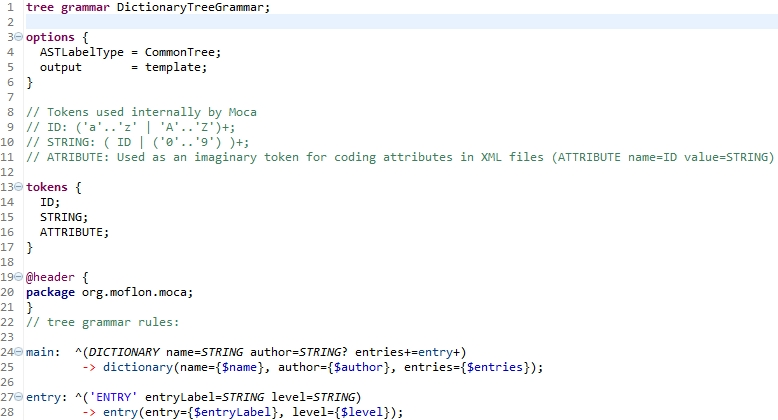
\includegraphics[width=\textwidth]{pics/moca/5MocaTreeToText/DictionaryTreeGrammar}
  \caption{Tree Grammar for the dictionary DSL} 
  \label{fig:moca-DictionaryTreeGrammar}
\end{center}
\end{figure} 

\item[$\blacktriangleright$] In the generated \texttt{src/org.moflon.org/dictionary/unparser/Dic\-tion\-ary\-Unparser\-Adapter.java} (Fig.~\ref{fig:moca-3-WizardResult}) a method for retrieving a group of templates has to be implemented.
Figure \ref{fig:moca-DictionaryUnparserAdapter} depicts the generated version showing how to use either a folder containing different template files, or a single file that contains all templates.
The latter is better for numerous smaller templates, while the former makes sense when the templates contain a lot of static text.
%\usepackage{graphics} is needed for \includegraphics
\clearpage 
\begin{figure}[!htbp]
\begin{center}
 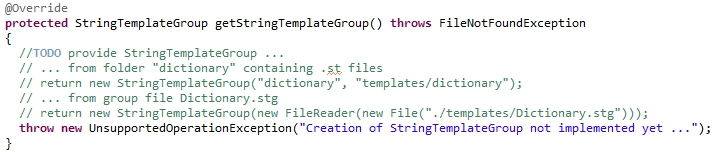
\includegraphics[width=0.87\textwidth]{pics/moca/5MocaTreeToText/UnparserAdapterNotImplemented}
  \caption{Unimplemented method getStringTemplateGroup} 
  \label{fig:moca-DictionaryUnparserAdapter}
\end{center}
\end{figure} 

For our small example a single file with all the templates is ideal, so uncomment the option for a \emph{group file}.
Your unparser adapter should now closely resemble Fig.~\ref{fig:moca-DictionaryUnparserAdapter}.  
 
\begin{figure}[!htbp]
\begin{center}
 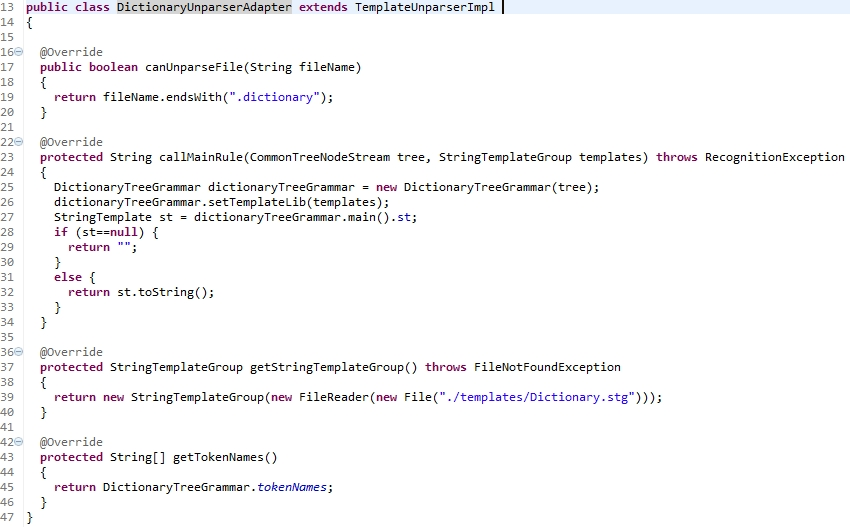
\includegraphics[width=\textwidth]{pics/moca/5MocaTreeToText/UnparserAdapter}
  \caption{Unparser Adapter} 
  \label{fig:moca-DictionaryUnparserAdapter}
\end{center}
\end{figure} 

\item[$\blacktriangleright$] The next step is to create the referenced template group file \texttt{Dic\-tion\-ary.stg} in \texttt{./templates}.
In this file, enter the contents depicted in Fig.~\ref{fig:moca-DictionaryTemplates}.    
ANTLR uses a template language called \emph{StringTemplate}.
StringTemplate is a very simple template language with few constructs and almost no constructs for complicated logic.
This might sound like a disadvantage but it actually prevents you from \emph{programming} in the templates and keeps them simple, readable and easily replaceable.
For further details about StringTemplate we refer to the website \url{www.stringtemplate.org}, a paper that argues for its simplicity \cite{PAR04}, and books on usage and features in combination with ANTLR \cite{ANTLR, LangImplPatterns}.
StringTemplate is pretty intuitive, take a good look at Fig.~\ref{fig:moca-DictionaryTemplates} and pay especially attention to how the templates are invoked in the tree grammar (Fig.~\ref{fig:moca-DictionaryTreeGrammar}).
You can easily make changes in the templates and see how it affects the generated files.
  %\usepackage{graphics} is needed for \includegraphics
\begin{figure}[!htbp]
\begin{center}
 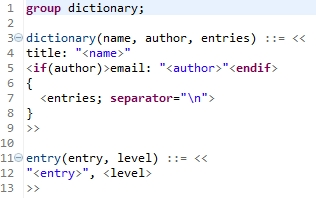
\includegraphics[width=0.5\textwidth]{pics/moca/5MocaTreeToText/DictionaryTemplates}
  \caption{Templates for the Dictionary DSL} 
  \label{fig:moca-DictionaryTemplates}
\end{center}
\end{figure} 

\item[$\blacktriangleright$] To complete the model-to-text transformation, open \texttt{MocaMain.java} (Fig.~\ref{fig:moca-8-MocaMain}) and edit lines 41-42 as follows:
\begin{verbatim}
// Perform tree-to-text
codeAdapter.unparse("instances", out);
\end{verbatim}
This calls the framework method \emph{unparse}, which creates a corresponding folder structure for a MocaTree instance and delegates code generation for each file using the registered unparsers.
This way different unparsers can be registered for different file types (defined by the unparser adapter's \texttt{canUnparseFile} method) and a whole folder structure containing different files can be generated.
Each parser can either use a single template group file like in our case, or a folder containing separated template files.

As we have always been updating our \texttt{MocaMain.java} file incrementally, Fig.~\ref{fig:moca-FinalMocaMain} shows the complete final version so you can compare before trying out the complete text-to-model and model-to-text round trip.

If you have done everything correctly, you should be able to run \texttt{MocaMain} and obtain similar results as depicted in Fig.~\ref{fig:moca-FinalResults}.
Note the created model \texttt{myLibrary.xmi} and the \texttt{.dictionary} files in \texttt{/out} that should now contain appropriate text in our DSL.
As a final test you can manipulate the model directly (e.g., create a new dictionary or shelf, add/delete an author) and adjust \texttt{MocaMain} appropriately so only the model-to-text transformation is performed.
Now compare the generated dictionaries to see if your changes are reflected correctly. 
 
%\usepackage{graphics} is needed for \includegraphics
\begin{figure}[!htbp]
\begin{center}
 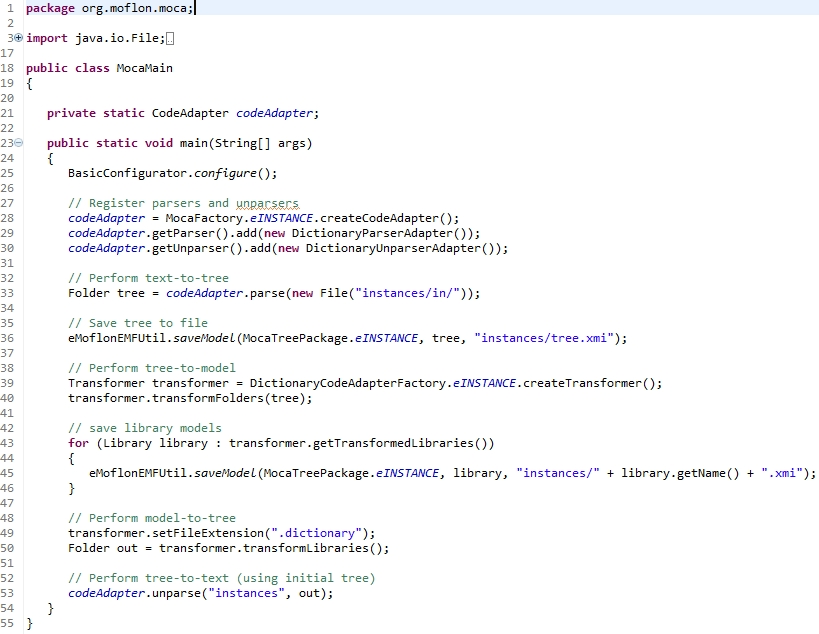
\includegraphics[width=\textwidth]{pics/moca/5MocaTreeToText/MocaMainComplete}
  \caption{Completed main method for Text-to-Model and Model-to-Text} 
  \label{fig:moca-FinalMocaMain}
\end{center}
\end{figure}

%\usepackage{graphics} is needed for \includegraphics
\begin{figure}[!htbp]
\begin{center}
 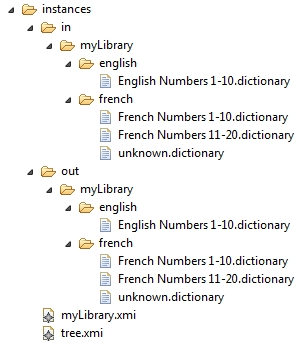
\includegraphics[width=0.5\textwidth]{pics/moca/5MocaTreeToText/InstancesAfterRoundTrip}
  \caption{Directory instances after parsing and unparsing.} 
  \label{fig:moca-FinalResults}
\end{center}
\end{figure}

\end{enumerate}